
\documentclass[11pt]{article}

% Packages
\usepackage[utf8]{inputenc}
\usepackage[T1]{fontenc}
\usepackage[margin=1in]{geometry}
\usepackage{graphicx}
\usepackage{xcolor}
\usepackage{tikz}
\usepackage{enumitem}
\usepackage{amsmath}
\usepackage{amsfonts}
\usepackage{hyperref}

% Custom colors
\definecolor{primaryblue}{RGB}{41, 128, 185}
\definecolor{accentgreen}{RGB}{39, 174, 96}
\definecolor{warningorange}{RGB}{230, 126, 34}
\definecolor{darkgray}{RGB}{52, 73, 94}

% Custom formatting
\setlength{\parindent}{0pt}
\setlength{\parskip}{6pt}

% Header formatting
\usepackage{fancyhdr}
\pagestyle{fancy}
\fancyhf{}
\fancyhead[L]{\color{primaryblue}\textbf{DataMender Project Proposal}}
\fancyhead[R]{\color{darkgray}Group 8}
\fancyfoot[C]{\thepage}

\begin{document}

% Title section
\begin{center}
    {\Huge\color{primaryblue}\textbf{DataMender: Smart Cleaning for Large CSV/Parquet Files}}
    
    \vspace{0.3cm}
    {\Large\color{darkgray}Project Proposal}
    
    \vspace{0.5cm}
    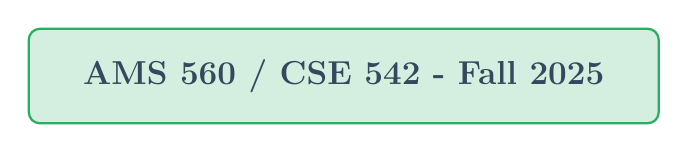
\begin{tikzpicture}
        \draw[accentgreen, thick, rounded corners, fill=accentgreen!20] (-4,-0.6) rectangle (4,0.6);
        \node[darkgray, font=\large\bfseries] at (0,0) {AMS 560 / CSE 542 - Fall 2025};
    \end{tikzpicture}
    
    \vspace{0.5cm}
    {\color{darkgray}\textbf{Team Members:}} \\
    Ahmad Javadi Nezhad • Daniel Bazmandeh • Iliya Mirzaei • Nicholas Tardugno • Tamali Halder
    
    \vspace{0.3cm}
    {\color{darkgray}September 2025}
\end{center}

\vspace{0.5cm}

% Section 1: Background and Motivation
\section{\color{primaryblue}Background and Motivation}

Data quality issues affect organizations working with large-scale datasets. Current solutions like OpenRefine require manual intervention, while Trifacta/Alteryx rely on rule-based transformations. However, \textbf{no existing tool uses Large Language Models (LLMs) for rule discovery} in large-scale data quality management.

Data scientists spend 60-80\% of their time on data cleaning tasks, yet lack automated tools that can suggest cleaning rules for multi-gigabyte datasets. This project addresses this need by combining data profiling with LLM-powered rule discovery and human validation.

% Section 2: Problem Statement and Importance  
\section{\color{primaryblue}Problem Statement and Importance}

\textbf{Core Problem:} Organizations struggle to efficiently clean large CSV/Parquet files due to lack of automated rule discovery systems that can handle multi-gigabyte datasets.

\textbf{Why This Matters:} Data cleaning consumes 60-80\% of data science workflows, manual rule creation doesn't scale to large datasets, existing tools lack LLM integration, and poor data quality leads to unreliable analytics and ML models.

\textbf{Target Use Case:} Ride-sharing companies with 5-10GB CSV files containing millions of records with inconsistent formatting, missing values, and data quality issues requiring cleaning rules.

% Section 3: Challenges
\section{\color{primaryblue}Challenges}

Key challenges include: (1) Profiling multi-gigabyte files efficiently without memory overflow, (2) Designing effective LLM prompts for rule discovery across different data types, (3) Creating UI tool for human validation, (4) Ensuring vectorized operations handle large-scale transformations, and (5) Balancing automated suggestions with human oversight.

% Section 4: Solution Approach
\section{\color{primaryblue}Solution Approach}

\textbf{DataMender} combines three key components:

(1) \textbf{Data Profiler:} Fast scanning using Pandas/NumPy/Dask to analyze row counts, column types, missing percentages, and histograms.

(2) \textbf{LLM Rule Discovery Engine:} Prompts that suggest range constraints, uniqueness checks, monotonicity validation, and sanity checks.

(3) \textbf{Human Validation:} UI tool for reviewing, accepting, editing, or rejecting suggested rules.


% Section 5: Deliverables and Timeline
\section{\color{primaryblue}Deliverables and Timeline}

\textbf{8-Week Timeline:} Weeks 1-2: Dataset selection and profiler implementation. Weeks 3-4: LLM prompt templates and UI tool. Weeks 5-6: Batch processing engine. Weeks 7-8: Polish, testing, and documentation.

\textbf{Final Deliverables:} (1) Working UI tool for data cleaning, (2) YAML configuration files with discovered cleaning rules, (3) Demonstration video showing complete workflow, (4) Technical report with performance metrics and lessons learned.

% Section 6: Division of Work
\section{\color{primaryblue}Division of Work Among Group Members}

\textbf{Ahmad Javadi Nezhad:} Project coordination, LLM integration, and rule discovery engine development.

\textbf{Daniel Bazmandeh:} Data profiler implementation and optimization.

\textbf{Iliya Mirzaei:} Validation UI design and UI interface development.

\textbf{Nicholas Tardugno:} Batch processing engine and data transformation implementation.

\textbf{Tamali Halder:} Testing, metrics collection, documentation, and final report preparation.

All members will contribute to dataset selection, testing, and final presentation preparation.

\textbf{Expected Impact:} DataMender will demonstrate how LLM-powered rule discovery can improve large-scale data cleaning workflows, providing a foundation for future research in AI-assisted data quality management.

\end{document}
